\documentclass[11pt, oneside]{article}
\usepackage{geometry}
\usepackage{graphicx}
\usepackage{amssymb}


\title{Is Florida getting warmer?}
\author{Xuan Wang}
\date{Oct 2022}

\begin{document}
\maketitle

\section{Introduction}

This document investigates whether Florida is getting warmer. 

The study is conducted against the null hypothesis of no significance is found between the year and the temperature in Florida.

\section{Results}

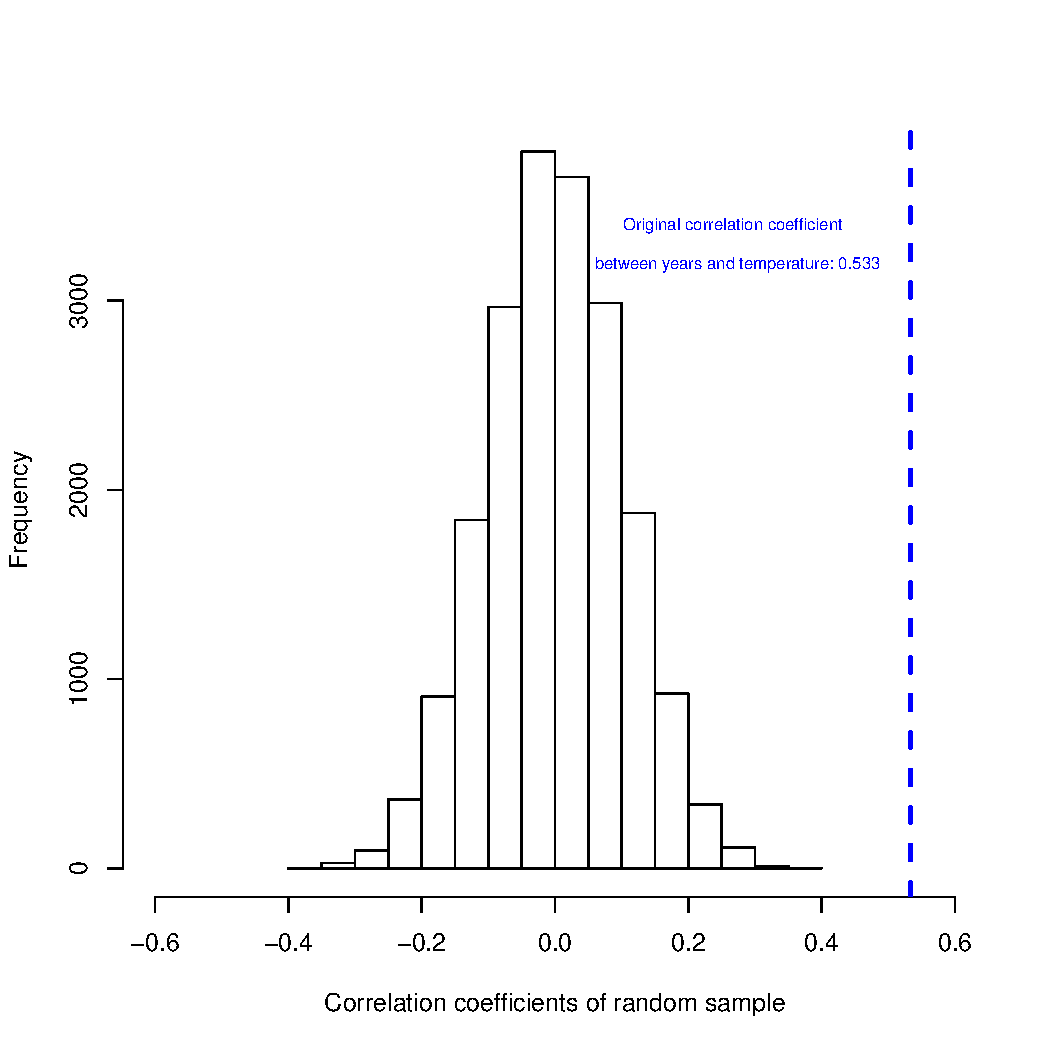
\includegraphics[scale = 0.5]{../results/Floridaplot.pdf}

\section{Interpretation}
To ensure the variables are independent, permutation analysis is conducted. Random correlation coefficients are generated and are compared with the observed coefficient, which is calculated to be 0.533.

According to the result, the p-value is 0 since there is no random correlation coefficients greater than the observed value.

This indicates that there is strong evidence to reject the null hypothesis. In this case, we conclude that the temperature in Florida is correlated with year.

\end{document}  
